
\section{Wörterbuchproblem}
Menge S mit n Schlüssln aus einem Universum U.
Operationen: INSERT (darauf achten, dass die Balance nicht verloren geht), DELETE, LOOKUP (Im Baum runterlaufen, bis das Element gefunden wurde)
\paragraph{Situationen}
\begin{enumerate}
    \item U linear geordnet, also existiert ein $ \leq $-Test $ \Rightarrow $ Suchbäume
    \item U ist ein Intervall $ \{0,..., N-1\} $ der gesamten Zahlen $ \Rightarrow $ Hashing
\end{enumerate}
\subsubsection{\underline{zu 1:}}

\paragraph{Randomisierte Suchbäume}
Idee: Benutze Zufallszahlen zur Balancierung eines binären Suchbaums

\paragraph{Binärer Suchbaum (Knoten-Orientiert)}
Schlüssel werden in den n Knoten eines binären Baums gespeichert, sodass im linken Unterbaum des Knotens mit Schlüssel x alle Schlüssel $ < x $ \textbf{und} im rechten Unterbaum alle $ > x $. Balanciert $ \Rightarrow Höhe(T)\leq logn$.  Degeneriert $ \Rightarrow Höhe(T) = O(n)$

\subsubsection{Definition: Randomized Search Tree (RST)}
Sei $ S=\{x_1,...,x_n\} $ eine Menge von n Schlüsseln. Jedem $ x_i $ wird eine zusätzlich eine Zufallszahl (auch Priorität genannt) $ prio(x_i) $ zugeordnet. $ prio(x_i) $ sind gleichverteilte reelle Zufallszahlen $ \in [0,1] $ (Implementierung wären int-Zahlen, zB 32-bit). \\
Ein RST für S ist eine binärer Suchbaum für die Paare $ (x_i, prio(x_i), 1 \leq i \leq n $, sodass
\begin{enumerate}
    \item normaler Knoten-orientierter Suchbaum für die Schlüssel $ x_i,...,x_n $
    \item Maximumsheap bzgl der Prioritäten. dh $ prio(v) \geq prio(u) $, falls v Parent. ((u,v) sind Knoten in einem Baum). $ \Rightarrow $ Wurzel enthält maximale Priorität.
\end{enumerate}
\textbf{Existenz} durch Algorithmus zum Aufbau (rekursiv).
\begin{itemize}
    \item Wurzel einthält $ (x_i, p_i) $ mit $ p_i = prio(x_i) $ maximal
    \item Linker Unterbaum: RST für $ \{(x_i, p_i)| x_j < x_i \} $
    \item Rechter Unterbaum: RST für $ \{(x_k, p_k)| x_k > x_i \} $
\end{itemize}
Beispiel: $ S=\{1,...,10\} $
\begin{itemize}
    \item Schreibe Tabelle mit Prioriäten und Werten.
    \item Teile die Tabelle beim Maximum und schreibe es in die Wurzel. Wiederhole, bis alle Elemente geschrieben.
\end{itemize}
$ \Rightarrow $ Wenn sich die Prioritäten genauso oder umgekehrt, wie die Schlüssel verhalten, erhält man einen degenrierten Baum. (bzgl $ \leq $). zB $ prio(x_i) = x_i $. Dieser Fall ist sehr unwahrscheinlich, wenn sich bei der Priorität um gleichverteilte Zufallszahlen handelt. 

\subsubsection{Operationen}

\begin{itemize}
    \item Lookup(x): normale suche in binärem Baum. Kosten $ O(Höhe(T)) $
    \item Insert(x): Füge einen neuen Knoten v als Blatt $ (x, prio(x)) $ gemäß des Schlüssels in den binären Baum ein, wobei $ prio(x) $ neue Zufallszahl (kann die Prio-Ordnung zerstören). Dann: Rotiere v nach oben, bis die Heap-Eigenschaft gilt, also $ prio(v) \leq prio(parent(v)) $. Kosten: O(\#Rotationen) = O(Höhe(T)). Alternativ: normales einfügen in binären Baum in absteigender Reihenfolge der Prioritäten.
    \item DELETE(x): Sei v der knoten mit Schlüssel x (v = Lookup(x)). Kosten: O(\#Rotationen) = O(1 + |L| + |R|)
    \begin{enumerate}
        \item Rotiere v nach unten, bis v ein Blatt ist. R = linkes Rückgrat des rechten Unterbaums von v. L = rechtes Rückgrat des linken Unterbaums. 
        \item Entferne das Blatt.
    \end{enumerate}
    \item Split(y) $ \rightarrow $ $ S_1=\{x\in S | x \leq y\}, S_2=\{x\in S | x \geq y\} $ (Teile den Baum, indem y mit maximaler Priorität zur Wurzel rotiert wird)
    \begin{enumerate}
        \item Insert($ y + \epsilon $) mit Priorität $ \infty $
        \item Entferne die Wurzel 
    \end{enumerate}
    \item Join$ (T_1, T_2 )$: $ S\leftarrow S_1 \cup S_2 $. $T_1$ RST für $S_1$ und $T_2$ RST für $S_2$
    \begin{enumerate}
        \item Konstruiere T (Füge y zwischen Max($S_1$) und Min($S_2$) ein. Voraussetzung: Max($S_1$) < Min($S_2$)
        \item Lösche die Wurzel (Durch runterrotieren des eingefügten Knotens y)
    \end{enumerate}
\end{itemize}

\subsubsection{Analyse des RST}
Wir analysieren die erwarteten Kosten einer Delete-Operation (Insert $ \rightarrow $ umgekehrtes Delete). Seit T ein RST für die Menge $ \{x_1,...,x_n\}mit x_1 < x_2 < ... < x_n $ der durch Inserts aufgebaut wurde. Bertrachte die Operation Delete($ x_k $) für eine $ k, 1\leq k\leq n $. Für einen Knoten $ x_k $ im Baum T mit Suchpfad $ P_k $, $ L_k $ rechtes Rückgrad von $ T_l $ und $ R_k $ linkes Rückgrad von $ T_r $.  Kosten $ O(|P_k| + |L_k| + |R_k|) $. Wir schätzen die Erwartungswerte 

\subsubsection{Lemma 1:}
\begin{itemize}
    \item a) E$ (|P_k|) $ = $ H_k + H_{n-k+1} - 1$ $$k-te\ Harmonische Zahl=H_k = \sum_{i_1}^{k}\frac{1}{i}\ H_k \leq ln(x)+1$$
    \item b) E$ (|L_k|) $ = $ 1-\frac{1}{k} $
    \item c) E$ (|R_k|) $ = $ 1-\frac{1}{n-k+1} $
\end{itemize}
\paragraph{Beweis} Betrachte eine Permutation $ \pi:[1..n] \rightarrow [1..n] $ (bijektive Abbildung), die die Schlüssel absteigend nach ihren Prio Werten sortiert. Dann gilt: 
\begin{enumerate}
    \item Jede Permutation $ \pi $ ist gleichwahrscheinlich (Wahrscheinlichkeit $ \frac{1}{n!} $), da die Prioritäten gleichverteilte Zufallszahlen sind.
    \item Man erhält den selben binären Baum durh einfügen der Schlüssel in einen unbalancierten Baum in der Reihenfolge, die $ \pi $ angibt. $ \rightarrow $ gleiches Vehalten, wie ein zufälliger binärer Baum.
    \item Baum wächst nur an den Blättern.
\end{enumerate}
Trick: arbeite ab jetzt mit zufälliger Permutation statt den Prioritäten. $ \rightarrow $ normaler Binärbaum mit zufälliger Einfügereihenfolge.
\paragraph{Teil a) des Lemmas} $P_k $ ist Suchpfad für Knoten $x_k $. Seien $ P'_k $ und $ P''_k $ Teilfolgen von $ P_k $ mit: $ \forall v \in P'_k, key(v)\leq x_k $ und $ \forall u \in P''_k, key(u)\geq x_k $. 
\begin{proof}
Beobachtungen:
\begin{enumerate}
    \item $ |P_k| = |P'_k| + |P''_k| - 1 $ ($ x_k $ in beiden Teilfolgen)
    \item $ P'_k = $ Menge der knoten v mit:
    \begin{itemize}
        \item Wenn v eingefügt wird, gilt key(v) ist maximal mit key(v)$ \leq x_k $
    \end{itemize}
    \item $ P''_k = $ Menge der knoten u mit:
    \begin{itemize}
        \item Wenn u eingefügt wird, gilt key(u) ist minimal mit key(u)$ \geq x_k $
    \end{itemize}
\end{enumerate}
Wir zeigen
\begin{enumerate}
    \item E($ |P'_k| $) = $ H_k $
    \item E($ |P''_k| $) = $ H_{n-k+1} $
\end{enumerate}
\underline{zu 1)} K mögliche Kandidaten für $ P'_k \{x_1,...,x_k\}$. Spiel: Ziehe zufällig Schlüssel aus $\{x_1,...,x_k\}$. E($ |P'_k| $) = Erwartungswert, wie of ein Kandidat gezogen wird, der $ \geq $ als alle vorher gezogenen ist (neues Maximum). $ A^k = E(|P'_k|)$ (Spiel A)

$$A^k = \sum_{i=1}^k \frac{1}{k} \cdot (1 + A^{k-i})$$

Im Zug $ x_i $ schließt $ x_1 ... x_i $ au. Dann gleiches Spiel mit K-i Kandidaten.

$$A^k = \frac{1}{k} (k + \sum^{k}_{i=1} A^{k-i}) $$
$$ = 1 + \frac{1}{k} \sum^{k}_{i=1} A^{k-i}$$ 

Wir zeigen durch Induktion über k, dass $ A^k = H_k $

\paragraph{IA}
$$ = 1 + \frac{1}{k} \sum^{k}_{i=0} H_i$$ 
Eigenschaften der harmonischen Zahlen:
\begin{enumerate}
    \item $$ \sum^{k}_{i=0} H_i = k \cdot (H_k -1 )$$
    \item $$ H_k \leq 1 + lnk$$ 
\end{enumerate}
aus 1) folgt: 

$$A^k = 1 + \frac{1}{k} \cdot k \cdot (H_k - 1)$$
$$    = 1 + H_k - 1$$
$$    = H_k$$
Der Erwartungswert ist ist gleich der k-ten Harmonischen Zahl. $E(P'_k) = H_k$. Abschätzung von $E(P''_k) =: B^k$. (Spiel B) kandidaten $ \{ x_k ... x_n\} $: Zähle, wie of ein neues Minimum gezogen wird. Dann sieht man leicht, dass 
$$B^k = H_{n-k+1}$$
Beweis: symmetrisch.
$$E(|P_k|) = E(|P'_k|) + E(|P''_k|) - 1 $$
$$ = A^k + B^k - 1 $$
$$ = H_k + H_{n-k+1} - 1 $$

\end{proof}

\paragraph{Teil b) des Lemmas}

\begin{proof}{$L_k$ und $R_k$}
Seien $ L_k = v_1, ... , v_l $ und $ R_k = u_1, ... , u_m $
\paragraph{Erwartungswerte}
Spiel C: Ziehe zufällig Elemente aus $ \{x_1 ... x_n \} $.
Sobald $ x_k $ gezogen wird: ??? Trigger ???
Sei $ C^k $ der Erwartungswert dieses Spiels, dh $ C^k = E(|L_k|) $.

$$ C^k = \frac{1}{k} \cdot A^{k-1} + \sum_{i=1}^{k-1} \frac{1}{k} \cdot C^{k-i}$$
im 1. Zug $ x_k $, dass Spiel mit k-1 Kandidaten (alle kleiner, als $ x_k $).

$$ C^k = \frac{1}{k} (\cdot H_{k-1} + \sum_{i=0}^{k-1} \cdot C^{i})$$

Trick: Schätze die Differenz zweier aufeinanderfolgender $ C^i $s = $ \delta_j = C^{j+1} - C ^j $ ab.

$$\Rightarrow C^k = \sum_{j=1}^k \delta_j + C^0$$

Beatrachte: 
$$ (j + 1) \cdot C^{j+1} - j \cdot C ^j $$
$$ = (j + 1) \frac{1}{j+1} (H_j + \sum_{i=0}^j C^i) - j \frac{1}{j} (H_{j-1} + \sum_{i=0}^j C^i)$$
$$ = H_j + \sum_{i=0}^j C^i - (H_{j-1} + \sum_{i=0}^j C^i)$$
$$ = H_j - H_{j-1} + C^i$$ 
$$ = \frac{1}{j} + C^j$$
Wir wissen nun, dass
$$ (j + 1) \cdot C^{j+1} - j \cdot C ^j  = \frac{1}{j} + C^j$$
$$ \frac{1}{j} = (j+1) C^{j+1} - (j+1) \cdot C^j $$
$$ \frac{1}{j(j+1)} = C^{j+1} - C^j = \delta_j $$
$$ \Rightarrow \delta_j = \frac{1}{j(j+1)} = \frac{1}{j} - \frac{1}{j+1}$$
$$ C^k = \sum_{j=1}^{k-1} \delta_j = \sum_{j=1}^{k-1} (\frac{1}{j} - \frac{1}{j+1})$$
$$ = 1 - \frac{1}{k}$$

\end{proof}


\paragraph{Teil c) des Lemmas}
Spiel $ D^k = E (|R_k|) $: Wie oft wird ein neues Minimum größer $ x_k $ gezogen, nachdem $ x_k $ gezogen wurde (Trigger).

\begin{proof}
symmetrisch:

$$ D^k = \frac{1}{n-k+1} \cdot B^{k-1} + \sum_{i=1}^{k-1 ??} \frac{1}{n+k-1} D^{i-k ??} $$
\textbf{...}
$$ D^k = 1 - \frac{1}{n-k+1}$$

\end{proof} 

\paragraph{Satz} Sie T ein RST für eine Menge von n Schlüsseln. Dann gilt:
\begin{enumerate}
    \item Die erwartete Laufzeit fpr Insert, Delete und Lookup ist O(logn)
    \item Die erwartete Zahl der Rotationen bei Delete ist < 2
\end{enumerate}
\paragraph{Beweis}
\begin{enumerate}
    \item Kosten von Lookup = $ O(|P_k|) $, Insert und Delete = $ O(|P_k| + |L_k| + |R_k|) $
    Kosten: $ O(H_k + H_{n-k+1} + 1 - \frac{1}{k} + 1- \frac{1}{n-k+1}) = O(H_n) = O(lnn) = O(logn)$
    \item Erwartete Zahl der Rotationen: $ E(|L_k|) + E(|R_k|) < 2 $
\end{enumerate}


\section{Hashing}

\subsection{Hashing mit offener Adressierung}
Tafel T $ [0, ..., m-1], m \leq n, |S| = n $
Verwende die Folge von Hashfunktionen $ h_0, h_1 $ 
$$ h_i(x) = f(x) + i \cdot g(x), i = 0,1,...$$
Häufig verwendet wird
$$ h_i(x) = (x \cdot mod m + i)\cdot mod m $$
$\rightarrow$ Linear Probing.\\
Idee
\begin{figure}[h]
    \begin{center}
        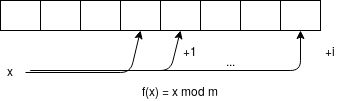
\includegraphics[width=10cm]{offeneadressierung.png}
        \caption{Idee: Offene Adressierungs-Tabelle}
        \label{fig:}
    \end{center}
\end{figure}

\paragraph{Operationen} Tafelposition T[i] belegt oder frei.
\begin{itemize}
    \item Init: alle frei
    \item Insert(x): betrachte die Tafelpositionen $T[h_0(x)], T[h_1(x)], T[h_2(x)]$ bis $ T[h_i(x)] $ frei und speicher x dort ab.
    $ T[h_i(x)] \leftarrow x $ und markiere $ T[h_i(x)]$ als belegt. Voraussetzungen:
    \begin{enumerate}
        \item $ m \leq |S| = n $
        \item $ h_i(x) $ frei $ i = 0,1,2,... $ muss alle Tafelpoitionen durchlaufen
    \end{enumerate}
    \item Lookup(x): Teste die Tafelpoition $ T[h_i(x)] $ für $ i=0,1,2,... $ bis entweder $ T[h_i(x)] = x $ erfolgreich oder $ T[h_i(x)] $ ist frei. \textbf{Terminiert nicht}, wenn m=n und die Tafel voll ist und das gesuchte Element nicht vorhanden ist. Daher idR $ m \geq n $
    \item Delete(x): (Idee 1):
    \begin{enumerate}
        \item $ j \leftarrow Lookup(x) $ 
        \item $ T[j] \leftarrow frei $, dann sind auf j folgende Elemente nicht mehr erreichbar.
    \end{enumerate}
    (Idee 2):
    \begin{enumerate}
        \item Dritter Zustand: 'gelöscht' (Details: Übung)
    \end{enumerate}
\end{itemize}



\subsection{Perfektes Hashing}
\textbf{Situation:} Statische Menge  S von n Schlüsseln aus $ [0,..,N-1] $. \textbf{Ziel:} Speichere S in einer Tafel der Größe O(n), sodass Lookup in Zeit O(1) realisiert werden kann (N >> n, N sehr viel größer, als n). \textbf{Andere Formulierung:} Finde einer Hashfunktion $ h: [0,..., N-1] \rightarrow [0,...,S-1] $ mit 
\begin{enumerate}
    \item S = Größe der Tafel und S = O(n)
    \item h injektiv auf S
\end{enumerate}
Zur Konstruktion oder Auswahl einer solchen Funktion Hashfunktion verwenden wir ein probabilitisches Verfahren (Zufallsverfahren).
\paragraph{Idee} 2-stufiges Hashing-Schema (Hashing-Verfahren)
\begin{figure}[h]
    \begin{center}
        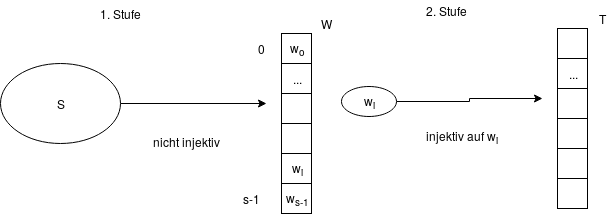
\includegraphics[width=10cm]{perfekthashing.png}
        \caption{Idee: Perfekt Hashing Tabellen}
        \label{fig:}
    \end{center}
\end{figure}

Sei p eine Primzahl mit p > N und $ S \in \mathbb{N} $ (Tafelgröße). Betrachte folgende Hashfunktionen:

$$ h_k:[0,...,N-1] \rightarrow [0,...,S-1] $$ mit $ h_k(x)= ((k \cdot x) mod p) mod s  $ für alle $ 1 \leq k \leq p-1 $ (Modulo Primzahl ergibt einen Restkörper, zB Inverses der Multiplikation). Diese Funktionen sind im Allgemeinen nicht injekt, dh $ h_k $ verteilt die Menge S auf s Buckets $ W_0^k, W_1^k, W_{s-1}^k $. 
$$ \Rightarrow W_i^k  = \{x\in S | h_k(x) = i\} $$

$ h_k $ injektiv auf $ S \Leftrightarrow |W_i^k| \leq 1 $ für $ 0 \leq i \leq s-1 $

\paragraph{Lemma 1: } Für jede Menge $ S \subseteq \{0,..., N-1 \}, |S| = n $ gilt $ \exists k, 1 \leq k \leq p-1 mit $

$$ \sum_{i=0}^{s-1} \binom{|W_i^k|}{2} < \frac{n^2}{s}$$
(Anzahl der Kollisionen < $\frac{n^2}{s}$). \\

\paragraph{Beweis} zunächst: Behauptung.
$$ \sum_{k=0}^{p-1} \sum_{i=0}^{s-1} \binom{|W_i^k|}{2} <  (p-1)\frac{n^2}{s}$$

Daraus folgt das Lemma (indirekt). Annahme, das Lemma 1 gilt nicht, dh $\forall 1\leq k\leq p-1: $

$$ \sum_{i=0}^{s-1} \binom{|W_i^k|}{2} \geq \frac{n^2}{s}$$

$$ \Rightarrow  \sum_{i=0}^{s-1} \binom{|W_i^k|}{2} \geq \frac{n^2}{s}$$
Widerspruch zur Behauptung!

\begin{proof}[Beweis zur Behauptung]

$$ (1)\sum_{k=0}^{p-1} \sum_{i=0}^{s-1} \binom{|W_i^k|}{2}$$
= Anzahl der Paare $ (k, \{x,y\} $, $ x\neq y$ und $ h_k(x) = h_k(y) $ (Anzahl der Kollisionen).\\
Wir schätzen zunächst den Betrag für 2 feste Werte $ x \neq y $ zur Behauptung ab.\\

Sei also $ x \neq y $: \\
(1) = Anzahl aller Ks mit $ (k\cdot x\cdot mod p)mods = (k \cdot y\cdot modp)mods $
\[ \Leftrightarrow ((k\cdot x\cdot mod p)-(k\cdot y\cdot mod p))mods = 0 \]
\[ k\cdot x\cdot mod p - k\cdot y\cdot mod p = i \cdot s \text{ für ein } i\in \mathbb{Z} \]
\[k\cdot (x-y) mod p = i\cdot s \]
Es gibt maximal $ \frac{2(p-1)}{s} $ mögliche Lösungen. Da p eine Primzahl ($ \mathbb{Z}_p $ ist ein Körper) hat jede dieser Gleichungen höchstens 1 Lösung für k.
$ \Rightarrow $ Beitrag eines festen Paares $ x \neq y $ zu (1) ist maximal $ \frac{2(p-1)}{s} $ \\

\[ \Rightarrow (1) \leq \binom{n}{2} \cdot \frac{2(p-1)}{s}\]
\[ = \frac{n(n-1)}{2} \cdot \frac{2(p-1)}{s}\]
\[ < \frac{n^2(p-1)}{s}\]

\end{proof}

\paragraph{Folgerung 1} (aus Lemma 1) \\
Für s=n (dh Tafel der Größe n): 
$$\exists k ,1 \leq k \leq p-1 \text{ mit } \sum_{i=0}^{n-1} |W_i^k|^2 < 3n$$

\begin{proof}[Beweis für Folgerung 1]
Betrachte Lemma 1 für s=n

\begin{flalign}
\exists k: \sum_{i=0}^{n-1}\binom{|W_i^k|}{2} &< n \\
\sum_{i=0}^{n-1} \frac{|W_i^k| \cdot(|W_i^k| - 1)}{2} &< n\\ 
\sum_{i=0}^{n-1} |W_i^k| \cdot(|W_i^k| - 1) &< 2 n \\
\sum_{i=0}^{n-1} |W_i^k|^2  &< 2 n + \sum_{i=0}^{n-1} |W_i^k|(=n) \\
 &<3n
\end{flalign}

\end{proof}


\paragraph{Folgerung 2} Für $ s = n^2 $ dh quadratische Tafelgröße. \\
$ \exists k' : 1\leq k \leq p-1 $, sodass die Hashfunktion
$$ k_{k'}:x \rightarrow (k'x\cdot modp) mods $$
injektiv auf S ist dh $ |W_i^k| \leq 1 \text{ für } 0\leq i \leq s-1 $.\\
$\Rightarrow$ Für Tafeln mit quadratische Größe existiert eine perfekte (injektive) Hashfunktion.

\begin{proof}[Beweis für Folgerung 2]
Betrachte Lemma 1 mit $ s= n^2 $

\begin{flalign}
\exists k': \sum_{i=0}^{n^2-1}\binom{|W_i^k|}{2} &< 1 \\
\Rightarrow  |W_i^k| &\leq 1\\
\Rightarrow  h_{k'}\text{ ist injektiv auf S}
\end{flalign}
(zu 6): dh Keine Kollisionen, bzw Doppeltbelegung in den $ W_i^k $

\end{proof}

Folgerung 2 zeigt Perfektes Hashing mit quadratischem Platz. Vermeidung des quadratischen Platzbedarfs durch ein 2-stufigen Hashing-Schema:

\begin{itemize}
    \item Stufe 1: Wähle ein k gemäß Folgerung 1, dh Tafelgröße s=n und Hashfunktion $ h_k $ mit $ \sum_{i=0}^{n-1} |W_i^k| < 3n $
    \item Stufe 2: Für jedes nicht-leere Bucket $ W_i^k $ der ersten Stufe verwende iene Tafel der Größe $ s_i = |W_i^k|^2 (0 \leq i \leq n-1) $ und wähle ein $k_i$ gemäß Folgerung 2, dh $ h_{k_i} $ ist injektiv auf $ W_i^k $
\end{itemize}

\begin{figure}[h]
    \begin{center}
        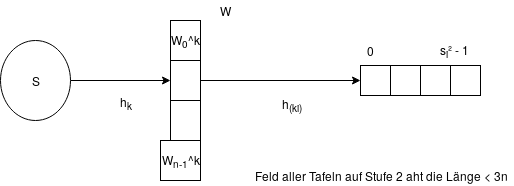
\includegraphics[width=15cm]{2stufenhashing.png}
        \caption{Konzept 2-Stufen Hashing}
        \label{fig:}
    \end{center}
\end{figure}


\subsubsection{Datenstruktur} 4 Felder + Variable k
\begin{itemize}
    \item Variable k: ($ h_k $ der 1. Stufe)
    \item k[0,...,n-1]: k[i] ist $ k_i $ der 2. Stufe
    \item Size[0,...,n-1]: Size[i] = $ |W_i^k| $ Bucketgrößen der 1. Stufe
    \item Ptr[0,...,n-1]: Pointer auf die Hashtafeln der 2. Stufe. Ptr[i] zeigt auf die Tafel B[0,...,Size[i]$^2$-1]
    \item T[0,...,3n]: Gesamtspeicherplatz aller B-Tafeln der 2. Stufe
\end{itemize} 

\begin{figure}[h]
    \begin{center}
        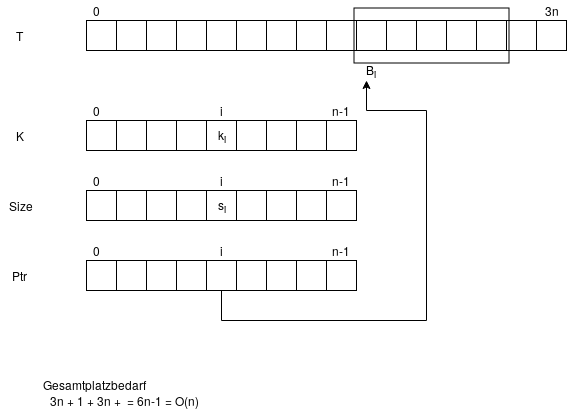
\includegraphics[width=15cm]{datenstruktur.png}
        \caption{Datenstruktur: Perfekt Hashing}
        \label{fig:}
    \end{center}
\end{figure}

\paragraph{Abspeichern eines Elements x}
\begin{flalign}
i &\leftarrow (k \cdot x mod p ) mod n\\
k' &\leftarrow K[i]\\
s' &\leftarrow Size[i]\\
j &\leftarrow (k'\cdot x mod p) mod s'\\
Ptr[i][j] &\leftarrow x
\end{flalign}

\begin{algorithm}
    
\end{algorithm}



\subsubsection{Aufbauzeit der Datenstruktur}
Wir findet man die k bzw k' Werte der ersten und zweiten Stufe (gemäß Folgerung 1 und 2). Aus Folgerungen 1 und 2 folgt: Es existiert immer mindestens ein Wert für k (dh eine geeignete Hashfunktion $ h_k $). \textbf{Aufbaualgorithmus:} Teste alle k-Werte. Auf 1. und 2. Stufe\\
\begin{algorithm}[H]
\SetKwProg{Def}{def}{:}{end}
\Def{Aufbau}{
    \For{$k=1$ \KwTo $p-1$} {
        1.Stufe: Teste ob $ \sum_{i=0}^{n-1} |W_i^k|^2 < 3n $\;
    }
}
\end{algorithm}
Kostet im worst case $ O(p \cdot n) = O(n \cdot N) $\\

2.Stufe für jedes Bucket $ W_i^k $ \\
\begin{algorithm}[H]
\SetKwProg{Def}{def}{:}{end}
\Def{Aufbau}{
    \For{$k'=1$ \KwTo $n$} {
        Teste ob $ h_{k'} \text{ injektiv auf } W_i^k$\;
    }
}
\end{algorithm}
Kostet für $ W_i^k O(p \cdot |W_i^k|$ für alle Buckets $ W_i^k (0 \leq i \leq n)$. Gesamtlaufzeit:

\begin{flalign}
O(\sum_{i=0}^{n-1} p\cdot|W_i^k|)    
\end{flalign}


Eine genauere Analyse zeigt, dass es viele  k-Werte mit den geforderten Eigenschaften gibt.

\paragraph{Folgerung 3} (aus Lemma 1) \\
Für mindestens die Hälfte aller k, $ 0 \leq k \leq p-1 $, gilt 
$$ \sum_{i=0}^{n-1}|W_i^k|^2 < 5n (s=n)$$

\paragraph{Folgerung 4} (aus Lemma 1) \\
Für mindestens die Hälfte aller k', $ 0 \leq k' \leq p-1 $, gilt 
$$ h_{k'}:x\rightarrow (k'\cdot x\ mod p) mod 2 \cdot  n^2 $$
ist injektiv auf S (angedwandt: $ W_i^ks $. Beweis analog zum Beweis der Folgerung 1 und 2.

\paragraph{Änderungen in der Datenstruktur} Auf 2.Stufe Tafelgrößen verdoppeln, dh jeweils Größe $ 2 \cdot |W_i^k|^2 $. Platzbedarf der 2.Stufe:

$$ \sum_{i=0}^{n-1} 2- |W_i^k|^2 = 2 \sum_{i=0}^{n-1} |W_i^k|^2 < 10n $$

Insgesamt: Platz 13n = O(n). 
\subparagraph{Aufbau}
\textbf{Stufe 1:} Wähle ein zufälliges $ k \in \{1,...,p-1 \} $ bis Folgerung 3 erfüllt. Wahrscheinlichkeit daür ist jeweils $ \geq \frac{1}{2} $. \textbf{Frage:} Wie hoch ist der Erwartungswert für die Anzahl der Tests. Analog zum Münzwurf: Wie viele Würfe, bis eine bestimmte Seite erscheint?
Erwartungswert für diese Zahl (Integrierende Reihe): 
$$ \sum_{i=0}^\infty \frac{1}{2^i} \cdot i = \frac{0.5}{(1-0.5)^2} = 2 $$
Erwartete Laufzeit für Stufe 1 ist dann $ O(2 \cdot |S|) = O(n) $. Analog für Stufe 2: Erwartete Zahl der Tests = 2. $ \Rightarrow $ Gesamtlaufzeit O(n).

\subsubsection{Zusammenfassung}
Man kann eine Menge S von n Schlüsseln aus $ [0,...,N-1] $ so abspeichern, dass gilt 
\begin{enumerate}
    \item Platubedarf ist O(n)
    \item Erwartete Aufbauzeit O(n)
    \item Zugriffszeit (Lookup) O(1) worst-case
\end{enumerate}

Dynamisierung ist möglich (Dynmaic Perfect Hashing). Idee: Zeigen, dass die gewählten k-Werte mit großer Wahrscheinlichkeit für weitere Schlüssel funktionieren.


\section{Planare Graphen}
Literatur: Nishizekim und Chiba (Planar Graphs). Graph kann in die Ebene gezeichnet werden, ohne dass sich Kanten kreuzen. Wir betrachten ungerichtete Graphen G=(V,E).
\subsection{Definition}
\begin{enumerate}
    \item Ein Graph G=(V,E) ist planar, wenn G eine planare Zeichnung hat.
    \item Eine planare Zeichnung von G ordnet jedem Knoten v einen Punkt $ p \in \mathbb{R}^2 $ (Ebene) zu, $ p = pos(x) $ heißt die Position von v, und jeder Kante $ (v,w) $ eine stetige Kurve im $ \mathbb{R}^2 $ mit den Endpunkten $ pos(v) $ und $ pos(w) $ zu, sodass sich diese Kurven paarweise nicht schneiden, außer in ihren Endpunkten. 
\end{enumerate}
G planar $ \Leftrightarrow $ $ \exists $ planare Zeichnung.
\paragraph{Beispiele}

\paragraph{nicht-planar} $ K_{3,3} $ bipartiter vollständiger Graph mit jeweils 3 Knoten auf jeder Seite. $ K_5 $ vollständiger Graph mit 5 Knoten. Ist ein Graph nicht planar, kann einer der beiden nicht-planaren Graphen gefunden werden.

\subsection{Planaritätstest}
Frage: ist der Graph planar?
\begin{enumerate}
    \item Falls planar: planare Zeichnung
    \item Falls nicht: möglichst kleiner nicht-planarer Teilgraph ($ K_{3,3} $ oder $ K_5 $)
\end{enumerate}

\paragraph{Beobachtung}
\begin{itemize}
    \item  G ist planar $ \Leftrightarrow $ $ \exists $ planare Zeichnung auf einer Kugeloberfläche
    \item Oberflächenstruktur von Polyedern kann durch planare Graphen dargestellt werden. (zB Würfel)
\end{itemize}

\subsection{Wichtige Begriffe und Definitionen}
\subsubsection{Kontenzusammenhang}
Der Zusammenhand eines Graphen (genauer Knotenzusammenhang).
\begin{itemize}
    \item G heißt einfach zusammenhängend, wenn es für jedes Paar $ (v,w) $ von Knoten einen Pfad zwischen v und w gibt. Zusammenhangskomponenten sind zusammenhängede Teilgraphen.
    \item G heißt zweifach zusammenhänged (biconnected), falls $ G \backslash \{v\} $ für jeden Knoten $ v \in V $ zusammenhängend ist. Der Knoten, der den Graph zerfallen lässt, nennt man Artikulationspunkt (cut-vertex)
    \item Ein zweifach zusammenhängeder Graph G heißt dreifach zusammenhänged, wenn für beliebige Knoten $ v,w $ gilt, $ G\backslash \{v,w\} $ ist zusammenhängend. Die Knoten, die den Graph zerfallen lassen nennt man Separationspaar. \textbf{Splitgraphen} $ G_1 $ und $ G_2 $ durch Entfernung eines Separationspaares, erweitert um Kopieen des Entferten Paares. Kante innerhalb des Separationspaares kann existieren oder nicht.
    \item Allgemein k-fach zusammenhängend kann man beliebige k-1 Knoten entfernen, sodass G zusammenhängend bleibt.
\end{itemize}
1-fach, 2-fach und 3-fach kann mit DFS in Zeit O(n+m) gelöst werden.

\subsubsection{Beobachtung} Ein nicht-zweifach zusammenhängender Graph G ist genau dann planaer, wenn seine zweifach Zusammenhangskomponenten (Blöcke) planar sind. \paragraph{Idee}
Konstruiere für jeden Block eine planare Zeichnung, sodass alle Cut-Vertices außen liegen und kleben diese zusammen.

\subsection{Planare Einbettung}
(Plane Graph) Abstrakte planare Zeichnung eines Graphen:
\begin{itemize}
    \item Keine Positionen (Koordinaten) für die Kanten
    \item Angabe der Flächen (Faces) in einer mögichen planaren Zeichnung 
\end{itemize}

% Graphik Faces
\begin{figure}[h]
    \begin{center}
        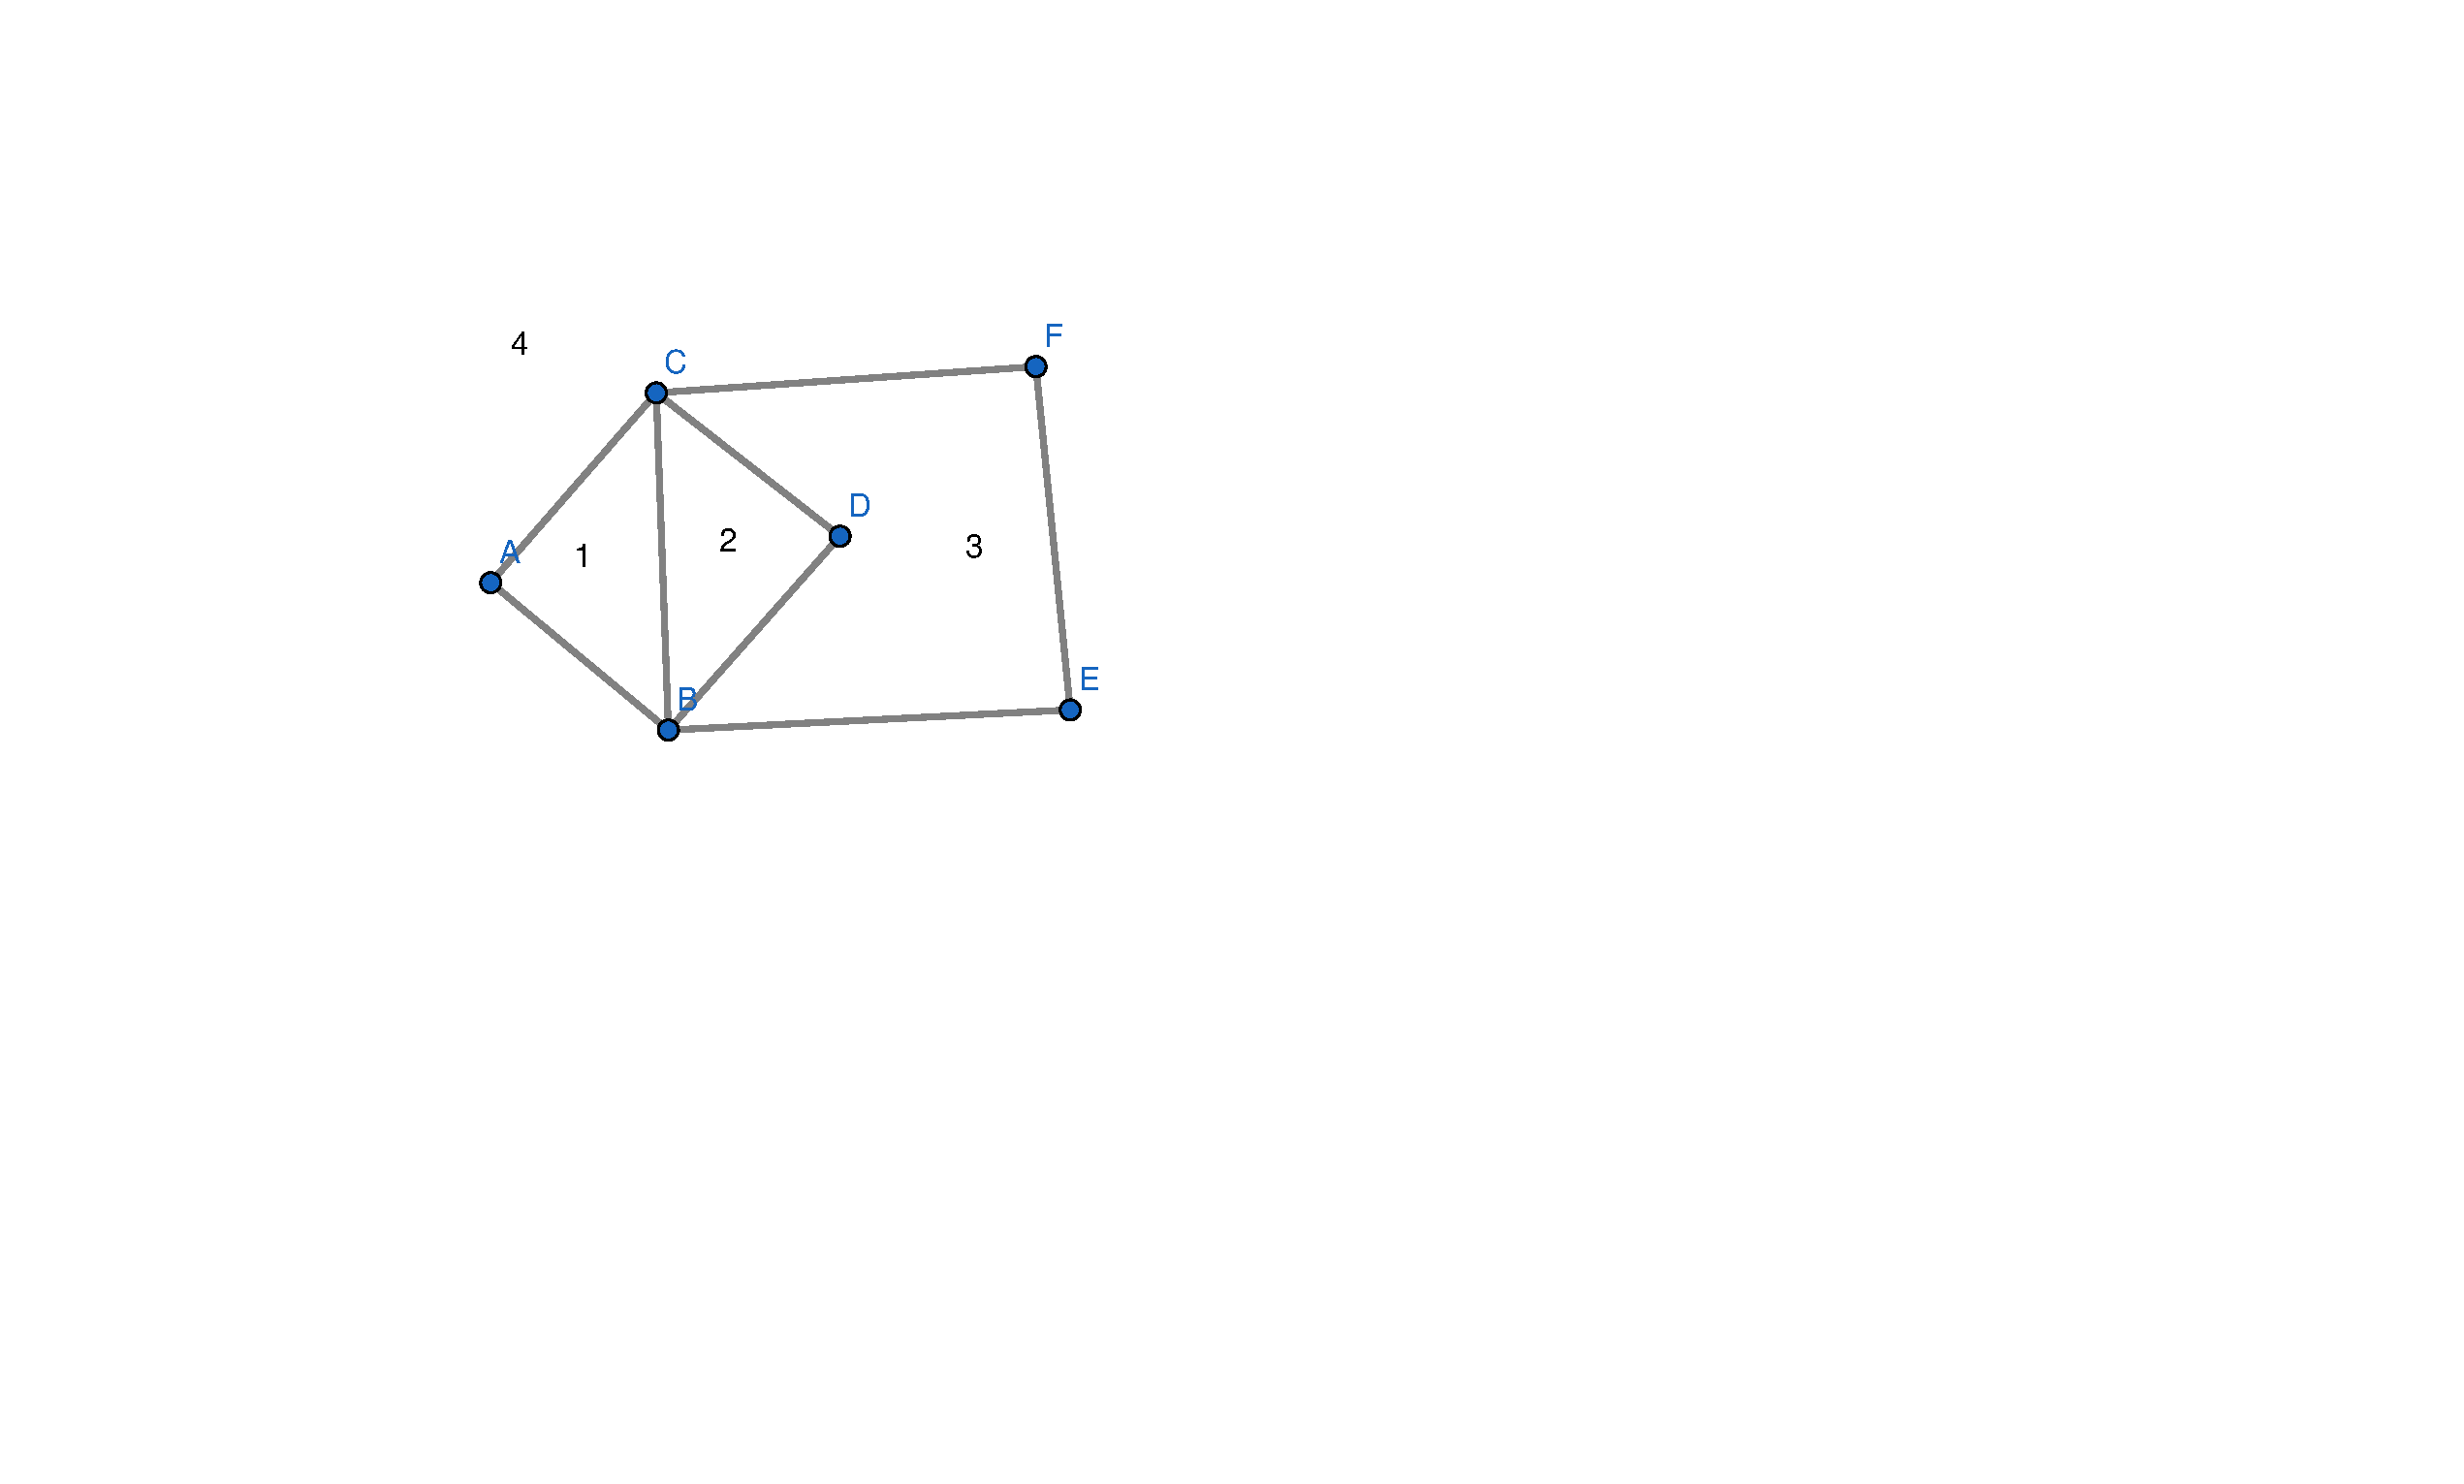
\includegraphics[width=15cm]{faces}
        \caption{Die Faces sind die Flächen, die durch die Kanten eingeschlossen werden.}
        \label{fig:}
    \end{center}
\end{figure}



\paragraph{Alternativ} Festlegung der Reihenfolge der Nachbarknotes jedes Knotens (Adjazenzliste) in einer möglichen planaren Zeichnung gegen den Uhrzeigersinn. Wir arbeiten meistens mit der 2. Alternative. Die beiden Definitionnen sind äquivalent.

\paragraph{Planaritätstest} bzw Einbettung besteht dann in der Aufgabe die Adjazenzlisten in eine Reihenfolge zu sortieren, so dass diese eine planare Einbettung definiert (falls möglich). Im Allgemeinen besitzt ein planarer Graph verschiedene panare Einbettungen (Hinweis: Einbettung ist eindeutig für 3-fach zusammenhängende Graphen). Beispiel für nicht-eindeutige Einbettungen (siehe Graphik). Die Faces sind die Flächen, die durch die Kanten eingeschlossen werden.

% Einbettung 
\begin{figure}[h]
    \begin{center}
        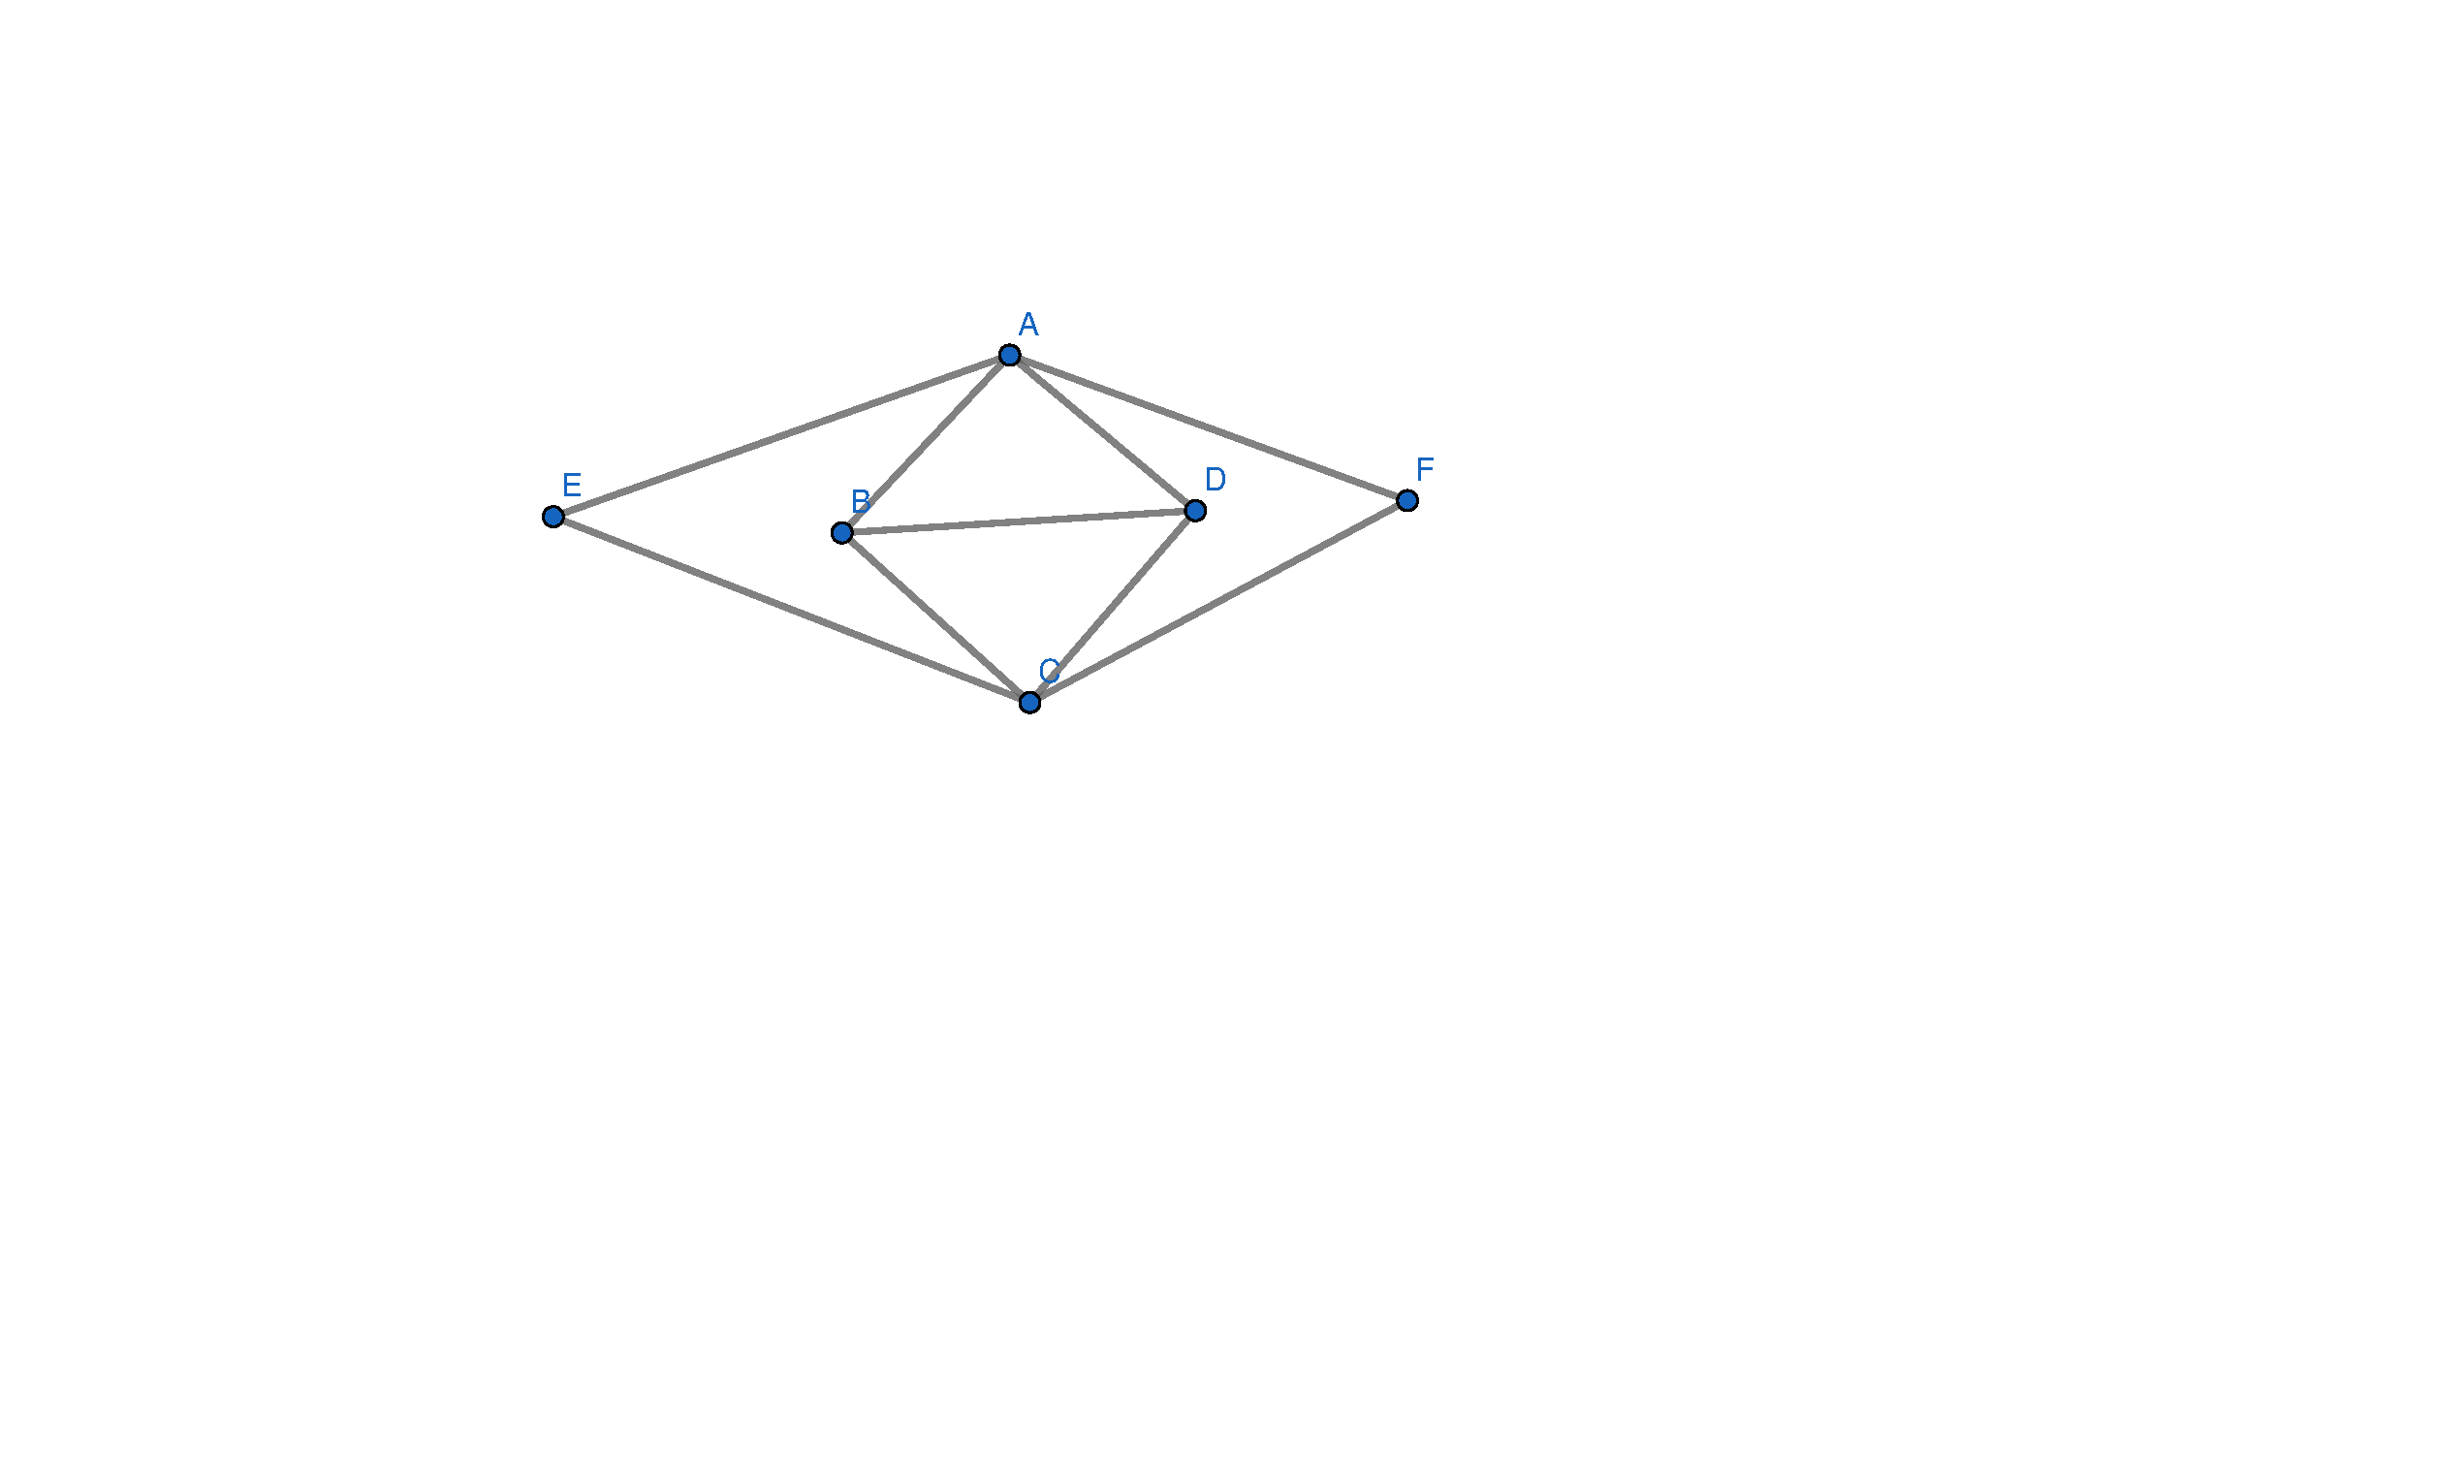
\includegraphics[width=15cm]{einbettung}
        \caption{Graph mit nichteindeutiger Einbettung: Rotation des unteren Teils (B und D)ergibt verschiedene Faces}
        \label{fig:}
    \end{center}
\end{figure}

\paragraph{Unterteilung (Subdivision)}
Sei G ein ungerichteter Graph. G' heißt Unterteilung oder Subdivision von G, wenn G' aus G durch ersetzen von Kanten durch Pfade entsteht (Platzieren neuer (Unterteilungs-)Knoten auf bestehende Kanten).

\subsection{Die Euler-Formel}
Sei G eine zusammenhängende planare Einbettung mit n Knoten, m Kanten und f Faces. Dann gilt
$$ n - m + f = 2 $$
\newpage
\begin{proof}[Euler-Formel]
Induktion über m\\
$\underline{m = 0:} $ Graph besteht aus einem isolierten Knoten: n=1, f=1  \\
$\underline{m > 0:} $ Sei G eine planare Einbettung mit m Kanten, n Knoten und f Faces \\
$\underline{IA} $ Für alle Einbettungen mit m-1 Kanten gilt die Formel \\
$\underline{Fall 1} $ G ist azyklisch (dh: Baum) 
\begin{enumerate}
    \item f = 1
    \item G besitzt Knoten v mit $ deg(v)=1 $ (Blatt)
\end{enumerate}
Die planare Einbettung $ G\backslash \{v\} $ ist zusammenhängend und hat n-1 Knoten und m-1 Kanten. 
$$ IA: (n-1) - (m-1) + f = 2 $$
$\underline{Fall 2} $ G ist kein Baum dh besitzt einen Kreis (f>1). Sei e eine beliebige Kante auf dem Kreis. Betrachte die planare Einbettung $ G\backslash \{e\} $

\begin{itemize}
    \item $ G\backslash \{e\} $ ist zusammenhängend
    \item $ G\backslash \{e\} $ hat m-1 Kanten, n Knoten und f-1 Flächen
\end{itemize}
$$ IA: n - (m-1) + (f - 1) = 2 $$

\end{proof}

\subsubsection{Folgerung}
Sei G ein planarer Graph 









